\documentclass{article}
\usepackage{graphicx}
\usepackage{amsmath}
\usepackage[margin=2cm, top=2cm]{geometry}
\usepackage{tikz}
  \usetikzlibrary{angles, quotes}
  \usetikzlibrary{arrows.meta}
  \usetikzlibrary{positioning}
\usepackage{pgfplots}
  \pgfplotsset{compat=1.18}
\usepackage{amssymb}
\usepackage{enumitem}
\usepackage{tocloft}
  \renewcommand{\cftsecdotsep}{\cftdotsep}
  \cftpagenumbersoff{subsection}
\usepackage[normalem]{ulem}
\usepackage{dashundergaps}
\usepackage{xcolor}
\usepackage[most]{tcolorbox}

\definecolor{defmain}{HTML}{1d1280}
\definecolor{defbg}{HTML}{F4F8F7}
\definecolor{rpmain}{HTML}{790a73}
\definecolor{rpbg}{HTML}{F5F5F8}
\definecolor{zgmain}{HTML}{146609}
\definecolor{zgbg}{HTML}{F4F6F8}

\newtcolorbox{defbox}[2][]{
    enhanced,
    colback=defbg,
    colframe=defmain,
    arc=3mm,
    boxrule=0.6pt,
    leftrule=1mm,
    before upper={\textbf{\sffamily\color{defmain}#2}\par\vspace{8pt}},
    #1
}

\newtcolorbox{rpbox}[2][]{
    enhanced,
    colback=rpbg,
    colframe=rpmain,
    arc=3mm,
    boxrule=0.6pt,
    leftrule=1mm,
    before upper={\textbf{\sffamily\color{rpmain}#2}\par\vspace{8pt}},
    #1
}

\newtcolorbox{zgledbox}[2][]{
    enhanced,
    colback=zgbg,
    colframe=zgmain,
    arc=3mm,
    boxrule=0.6pt,
    leftrule=1mm,
    before upper={\textbf{\sffamily\color{zgmain}#2}\par\vspace{8pt}},
    #1
}

\title{Zapiski za MAT v 3. letniku}
\author{Gašper Mikložič}
\date{}

\begin{document}

\maketitle

\section{Kvadratna neenačba}

\begin{defbox}{Definicija}
    \centering \large
    Enačba oblike:
    $$ ax^2 + bx + c > 0 $$
    $$ ax^2 + bx + c < 0 $$
    $$ ax^2 + bx + c \leq 0 $$
    $$ ax^2 + bx + c \geq 0 $$ \\
    Kjer $a$ \neq 0.\\ 
    Rešitev neenačbe je interval, unija intervalov ali prazna množica.
\end{defbox}

\begin{zgledbox}{Način reševanja}
    \centering
    $2x^2 < -4x + 8$\\
    $2x^2 +4x -8 < 0$\\
    $x^2 + 3x - 4 < 0$\\
    Tukaj rešimo kot kvadratno enačbo,\\ z Vietovim pravilom ali formulo za kvadratno enačbo.\\
    $x_1=-4$\\
    $x_2=1$\\
    Nato zapišemo interval. Če je znak je manjše(kot v tem primeru)\\ zapišemo interval, kdaj graf funkcije leži pod abscisno osjo.\\ Če je znak večje, zapišemo, kdaj graf leži nad abscisno osjo. Dobimo rešitev.\\[1mm]
    \large \boxed{$x \in (-4, 1)$}
\end{zgledbox}

\newpage

\section{Kompleksna števila}

\begin{defbox}{Definicija}
    \centering
    Komplesna števila, označena s simbolom $\mathbb{C}$, so vsa števila, ki jih lahko opišemo s predpisom:\\[8pt]
    $z=a+bi$\\[8pt]
    Kjer sta $a$ in $b$ realni števili in je $i^2$ enak $-1$\\[10pt]
    Vsako število lahko tudi razdelimo na realno in imaginarno komponento:\\
    $\text{Re}(z)=a$ in $\text{Re}(z)=b$
\end{defbox}

\begin{rpbox}{Graf}
    \centering
    Vsa kompleksna števila lahko tudi ponazorimo na grafu\\ kjer je abscisna os realna komponenta in ordinatna os imaginarna komponenta.
    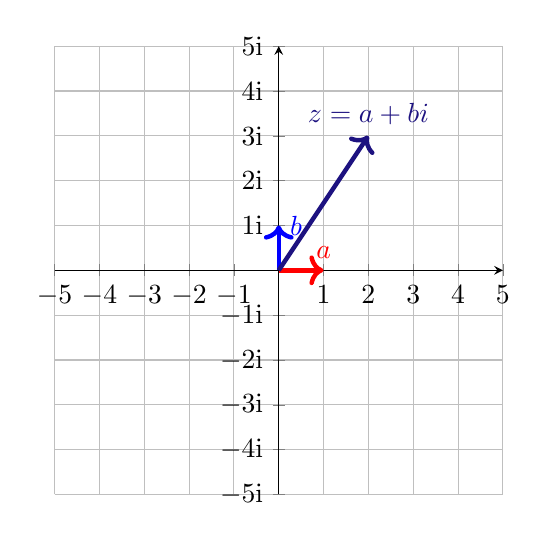
\begin{tikzpicture}[scale=1]
    \begin{axis}
        [
        axis lines = middle,
        grid = both,
        xmin = -5, xmax = 5,
        ymin = -5, ymax = 5,
        xtick={-5,...,5},
        ytick={-5,...,5},
        yticklabel={\pgfmathprintnumber{\tick}i},
        unit vector ratio=1 1 1
        ]
        \coordinate (O) at (0,0);
        \coordinate (I) at (1,0);
        \coordinate (J) at (0,1);
        \coordinate (Z) at (2,3);
        \draw[->,red,ultra thick] (O) -- (I) node[above] {$a$};
        \draw[->,blue,ultra thick] (O) -- (J) node[right] {$b$};
        \draw[->,defmain,ultra thick] (O) -- (Z) node[above] {$z=a+bi$};
    \end{axis}
\end{tikzpicture}
\end{rpbox}

\end{document}